\anonsection{Задание 4}
\anonsubsection{Формулировка задания}
\begin{enumerate}
\item Построить датчик распределения Коши. 
\item На основе датчика распределения Коши с помощью метода фон Неймана построить
 датчик стандартного нормального распределения. При помощи функции normal
 probabitity plot убедиться в корректности построенного датчика и обосновать
 наблюдаемую линейную зависимость.
\item Сравнить скорость моделирования стандартного нормального распределения в
 заданях 3 и 4.
\end{enumerate}

\anonsubsection{Датчик распределения Коши}
\begin{definition}
	Случайная величина $X$ имеет распределение Коши с параметрами $a$ и $b$, если
     ее функция распределения имеет вид:
    $$
	F_X(x) = \frac{1}{\pi}\arctan\left(\frac{x - a}{b}\right) + \frac{1}{2}.
	$$
	Плотность распределения Коши:
	$$
	p_X(x) = \frac{1}{\pi}\frac{b}{(x- a)^2 + b^2}.
	$$
\end{definition}

Функция распределения $F_X(x)$ обладает обратной, а значит в данном случае для
 моделирования распределения можно пользоваться методом обратной функции
 (Теорема \eqref{theor_inverse}). Обратная функция для $F_X(x)$ равна $F_X^{-1}(y)
 = a + b\tan\left(\pi\left(y - \frac{1}{2}\right)\right)$. Следовательно,
 в качестве датчика распределения Коши можно построить датчик случайной величины
 $X = F_X^{-1}(Y)$, где $Y \sim U[0, 1]$. На Рис.\eqref{fig:cauchy_ecdf}
 продемонстрировано совпадение эмпирической и теоретической функций распределения
 для распределения Коши, полученного построенным датчиком.

\begin{figure}[ht]
	\centering
	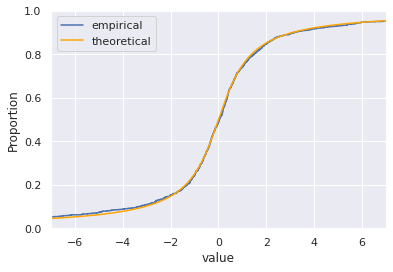
\includegraphics[width = 0.7\linewidth]{"./resources/cauchy_ecdf.png"}
	\caption{Демонстрация совпадения эмпирической и теоретической функций
     распределения для распределения Коши. Размер выборки: $ n = 1000 $.}
    \label{fig:cauchy_ecdf}
\end{figure}

\anonsubsection{Метод фон Неймана}
Метод фон Неймана заключается в моделировании нормального распределения путём
 мажорирования плотностью распределения Коши с параметрами $a$ и $b$. Для достижения
 наилучшей оценки, будем подбирать параметры $a$ и $b$. \\
Плотность стандартного нормального распределения $p_1(x)$ и плотность распределения
 Коши $p_2(x)$ выглядят следующим образом:
$$
    p_1(x) = \frac{1}{\sqrt{2\pi}}e^{-\frac{x^2}{2}},
$$

$$
    p_2(x) = \frac{1}{\pi}\frac{b}{(x - a)^2 + b^2}.
$$

При моделировании будем следовать алгоритму:
\begin{enumerate}
	\item возьмем некоторое число $k > 0$, такое что $p_1(x) \leq kp_2(x),
     \forall x\in \mathbb{R}$,
	\item рассмотрим значение случайной величины $x = X, X\sim Cauchy(a, b)$,
	\item сгенерируем случайную величину $y = Y(x)\sim Bern\left(\frac{p_1(x)}
     {kp_2(x)}\right)$,
	\item если $y = 1$, то $x$ --- значение из распределения с плотностью $p_1(x)$,
     иначе --- продолжаем моделирование, начиная с пункта 2).
\end{enumerate}
Данный алгоритм работает тем быстрее, чем ближе отношение $\frac{p_1(x)}{kp_2(x)}$
 к единице, поэтому в качестве $k$ возьмем $k^* = \min\limits_{a, b}
 \max\limits_x\frac{p_1(x)}{p_2(x)}$.
Рассмотрим отношение 
$$
    \frac{p_1(x)}{p_2(x)} = \frac{\sqrt{\pi}}{\sqrt{2}b}e^{-\frac{x^2}{2}} 
     \left((x - a)^2 + b^2\right).
$$
Пусть $a = 0$. Рассмотрим вспомогательную функцию:
$$
    g(x) = e^{-\frac{x^2}{2}} \left( x^2 + b^2 \right).
$$
Найдем максимум этой функции:
$$
    g'(x) = e^{-\frac{x^2}{2}} x \left( 2 - b^2 - x^2 \right) = 0,
$$
следовательно, точки экстремума:
$$
    \left[
    \begin{aligned}
        x = 0, |b| > \sqrt{2},\\
        x = \pm\sqrt{2 - b^2}, 0 < |b| \leq \sqrt{2}.
    \end{aligned}
    \right.
$$
Таким образом,
$$
    k* = \min \left\{ \min_{|b| > \sqrt{2}} \sqrt{\frac{\pi}{2}} b,\;
     \min_{0 < |b| < \sqrt{2}} \frac{\sqrt{2\pi}}{b}e^{\frac{b^2}{2} - 1} \right\}.
$$
Поскольку $k > 0$, то и $b > 0$. Найдем максимум вспомогательной функции
$$
    h(b) = \frac{e^{\frac{b^2}{2} - 1}}{b}:
$$

$$
    h'(b) = \frac{1-b^2}{b^2}e^{\frac{b^2}{2} - 1},
$$

следовательно, поскольку $b > 0$, точкой экстремума является $b = 1$.\\
Получаем оптимум при $a^* = 0,\, b^* = 1:$
$$
    k^* = \min\left\{\sqrt{\pi}, \sqrt{\frac{2\pi}{e}}\right\} = 
     \sqrt{\frac{2\pi}{e}}.
$$
Докажем, что $a = 0$ --- оптимальное значение параметра.
\begin{multline}
    k^* = \min_{a, b} \max_x \left( \frac{\sqrt{\pi}}{\sqrt{2}b} e^{-\frac{x^2}{2}}
     \left((x - a)^2 + b^2\right)\right) = \\
    = \min_a\left\{\min_{b > \sqrt{2}}\left.\frac{p_1(x)}{p_2(x)}\right|_{x = 0},
     \left.\min_{0 < b\leq\sqrt{2}}\frac{p_1(x)}{p_2(x)}\right|_{x =
     \pm\sqrt{2 - b^2}}\right\} > \\
    > \min_a\left\{min_{b > \sqrt{2}}\frac{\sqrt{\pi}}{\sqrt{2}b}
     \left(a^2 + b^2\right), \min_{0 < b \leq \sqrt{2}} \left( \sqrt{2 - b^2} +
     |a|\right)\right\}
\end{multline}
Минимум выражения достигается при $a = 0$.

Иллюстрация работы построенного датчика, использующая Python функцию
 scipy.stats.probplot, представлена на Рис. \eqref{fig:norm_probplot}. На оси ординат
 откладываются точки выборки, на оси абсцисс --- квантили стандартного нормального
 распределения. Прямой линии соответствует "точное"  нормальное распределение,
 наилучшим образом приближающее, в смысле указанных осей, значения выборки. Видно, 
 что полученная с помощью датчика Фон-Неймана выборка следует стандартному нормальному
 распределению.

\begin{figure}[ht]
	\centering
	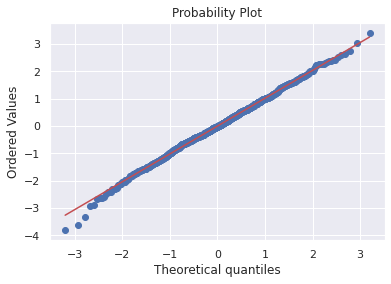
\includegraphics[width = 0.7\linewidth]{"./resources/norm_probplot.png"}
	\caption{Демонстрация совпадения построенного с помощью метода Фон-Неймана
     распределения со стандартным номральным при размере выборки $ n = 1000 $.}
    \label{fig:norm_probplot}
\end{figure}

 Возьмем далее случайную величину  \( \xi\sim N(\mu,\sigma^2) \). Ее функция
 распределения
$$
	F_{\xi}(x) = \dfrac{1}{\sqrt{2\pi\sigma^2}} \int\limits_{-\infty}^x
     e^{-\dfrac{(t - \mu)^2}{2 \sigma^2}} dt
$$
Введем замену переменной $ s = \dfrac{t - \mu}{\sigma} $. Тогда
$$
	F_{\xi}(x) = \dfrac{1}{\sqrt{2\pi}} \int\limits_{-\infty}^{\frac{x - \mu}
     {\sigma}} e^{-\dfrac{s^2}{2}} ds = F \left( \dfrac{x - \mu}{\sigma} \right) 
$$
где \( F(x) \) --- функция стандартного нормального распределения.

Таким образом, квантили различных распределений связаны между собой линейно, что
 означает, что любую нормальную случайную величину \( \xi \sim N(\mu, \sigma^2) \)
 можно представить в виде \( \xi = \sigma \eta + \mu \), где \( \eta \sim N(0,1) \),
 а прямая в функции probplot будет прямой со сдвигом \( \mu \) и с коэффициентом
 наклона \( \sigma \).

\anonsubsection{Сравнение времени работы}
На Рис. \eqref{fig:times} приведен график сравнения скорости работы датчика
 стандартного нормального распределения с моделированием случайных величин парами
 и датчика, построенного методом Фон-Неймана.

\begin{figure}[ht]
	\centering
	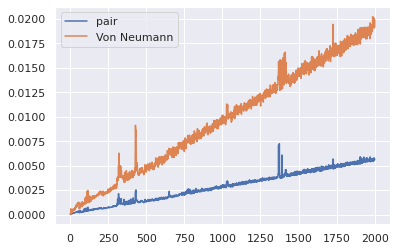
\includegraphics[width = 0.7\linewidth]{"./resources/times.png"}
	\caption{Зависимость времени моделирования от размера генерируемой выборки.}
    \label{fig:times}
\end{figure}